\chapter{Evaluation}

As part of our work we prepared and performed series of experiments using eZ430.
This chapter describes the motivation, methodology and results of those tests.  

\section{Power usage}

\subsection{Official specification}
Texas Instruments provide a specification of eZ430 power usage (Table \ref{tab:power-specification}).
It contains detail data about sensor measurement power usage and during pre-build eZ430 applications: BlueRobin and SimpliciTI.
Both of this apps are controlled from PC using Chronos Control Center (Figure \ref{fig:chronos_control_center}).

\begin{figure}[h]
  \centering
  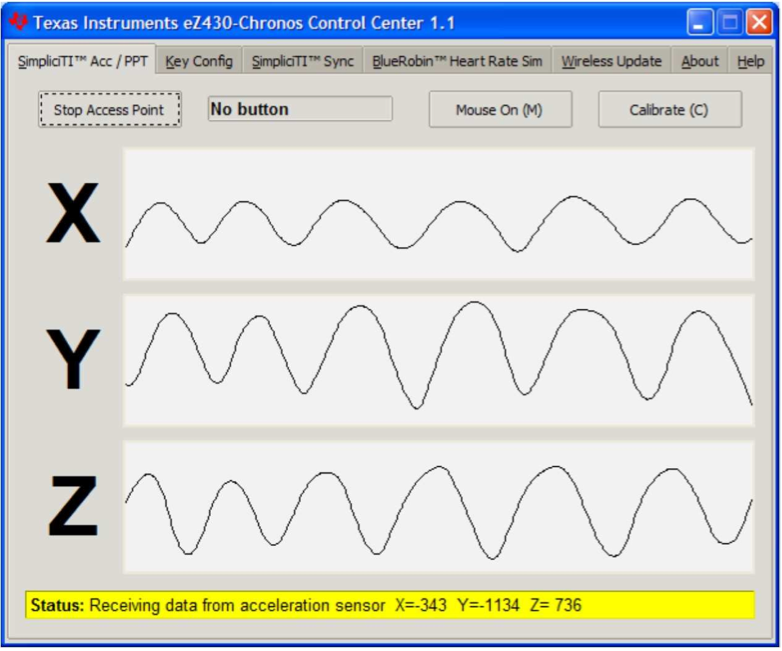
\includegraphics[width=0.6\textwidth]{img/chronos_app_control_center.png}
  \caption{Chronos Control Center PC Software (Courtesy of Texas
  Instruments)}
  \label{fig:chronos_control_center}
\end{figure}


\begin{table}
  \centering
    \begin{tabular}{|l|r|r|}
        \hline
        \textbf{Mode} & \textbf{Average Current} & \textbf{Battery Life} \\ \hline
        Shelf mode (LPM4) & 2.7 $\mu A$ & 92.6 months \\ \hline
        Welcome screen (LPM3) & 8.9 $\mu A$ & 28.0 months \\ \hline
        Time/Date & 9.0 $\mu A$ & 27.7 months \\ \hline
        Continuous temperature measurement & 10.0 $\mu A$ & 25.0 months \\ \hline
        Continuous altitude measurement & 18.0 $\mu A$ & 13.8 months \\ \hline
        Continuous acceleration measurement & 166.0 $\mu A$ & 1.5 months \\ \hline
        Continuous BlueRobin RX & 40.0 $\mu A$ & 6.2 months \\ \hline
        Continuous SimpliciTI PPT (no button pressed) & 10.0 $\mu A$ & 25.0 months \\ \hline
        Continuous SimpliciTI SYNC & 0.9 $m A$ & 8 days \\ \hline
        Continuous SimpliciTI ACC & 3.7 $m A$ & 2 days \\ \hline
        1h/day BlueRobin RX & 10.3 $\mu A$ & 24.2 months \\ \hline
        1h/day SimpliciTI PPT (no button pressed) & 9.1 $\mu A$ & 25.4 months \\ \hline
        1h/day SimpliciTI SYNC & 46.1 $\mu A$ & 5.4 months \\ \hline
        1h/day SimpliciTI ACC & 169.9 $\mu A$ & 1.4 months \\ \hline
    \end{tabular}
  \caption{eZ430 Chronos estimated battery life (from Texas Instrument User's Guide, p. 64)}
  \label{tab:power-specification}
\end{table}

BlueRobin\footnote{BlueRobin is a trademark of BM innovations GmbH} simulate active heart belt.
It periodically transfer heart beat, speed and distance through radio to PC.

SimpliciTI\footnote{SimpliciTi is a trademark of Texas Instrument} is a versatile tool.
It consist of several modes.
PowerPoint Control mode (PPT) allows to map eZ430 buttons to PC keys.
That way user could control presentation, music player, etc.
Acceleration data mode (ACC) transmit eZ430 acceleration data to PC through radio.
It is also possible to control PC mouse using those data.
Synchronization mode (SYNC) allows to calibrate device sensors and set the time on eZ430 from PC.
In addition to that, SimpliciTI provides standard watch functionality such as clock, timer, alarm, etc. 

Unfortunately, the important details, such as duty cycle and radio transfer rate are not specified for both applications.
Moreover, there are no data about most power intensive operations - receiving and sending the radio packets.
Both of this operations consume orders of magnitude more energy, so having the detail measurements is required to do accurate estimations.

\subsection{Test setup and methodology}

\begin{figure}[h]
  \centering
  \includegraphics[width=0.4\textwidth]{diagrams/power.eps}
  \caption{Power measurement setup}
  \label{fig:power}
\end{figure}

% schema
Though, we do not have a device which could measure electric current directly over time, we were able to calculate current indirectly using Ohm's Law: 

$$
U = I \cdot R
$$

It states that the potential difference on resistor (U) is equal to current (I) divided by resistance (R).
In our setup we know the resistance of resistor in Ohm and could measure voltage drop using oscilloscope (Figure \ref{fig:power}).
So using formula:

$$
I = \frac{U}{R}
$$

We are able to calculate current.


In addition to that, in physical world there is additional voltage drop caused by resistor.
So we have to subtract it from final calculations.

The Oscilloscope Owon PDS 5022S was used (Figure \ref{fig:owon}.
It is capable of plotting voltage difference with $< 0.1 ms$ accuracy.

\begin{figure}[h]
  \centering
  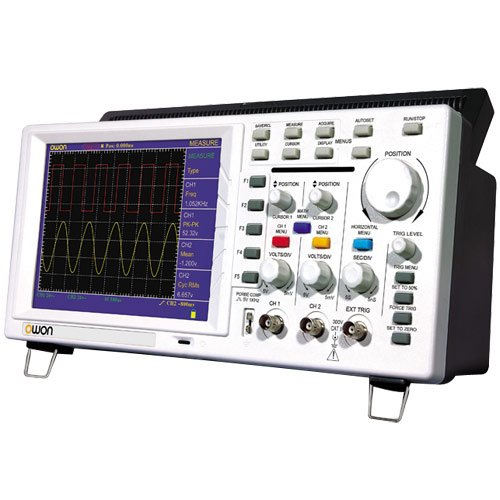
\includegraphics[width=0.4\textwidth]{img/owon_pds5022s.jpg}
  \caption{Owon PDS5022S Oscilloscope (courtesy to the manufacturer)}
  \label{fig:owon}
\end{figure}

Having that setup we run series of tests.
Each one begins with programming eZ430 with special purpose application described in Table \ref{tab:power-apps}.
Every application run for a few minutes, pausing the plot several times and recording the voltage difference.
Also a video was recorded for verification purposes.
As a final measure we take average of observations and round it to 1 $ mV $.

For most of the tests the the voltage drop was almost constant, but we could send radio packets with certain frequencies.
So sending power consumption was measured only when actual packets were sent.

Similar issue exists in low-power listening, where we measured the top power consumption and other parameters described in one of the next paragraphs.


\begin{table}
  \centering
    \begin{tabular}{|l|l|}
        \hline
    \textbf{Application} & \textbf{Description} \\ \hline
    Null app & sleeps all the time \\ \hline
    LCDDriverTest App & uses LCD display intensively \\ \hline
    Loop & perform the computations at maximal speed without sleeping \\ \hline
    TestAccelerator & Reads in a loop the acceleration reading, \\
    & unintentionally it is also maxing out CPU \\ \hline
    Radio listening & listen on radio (no difference whether it gets packets) \\ \hline
    Low-power listening & wakes every X $ ms $ to check if someone transmit on radio \\ \hline
    Sending at maximal power & sends packets with strongest signal - at +12 $ dB $ \\ \hline
    Sending at minimal power & sends packets with weakest signal - at -30 $ dB $ \\ \hline
    \end{tabular}
  \caption{Special purpose application used while measuring currency}
  \label{tab:power-apps}
\end{table}

\subsection{Results}

Our equipment was good enough to measure radio related operations with reasonable accuracy (Table \ref{tab:power-usage}).
Contrary, the onboard sensors consume too little energy to be above the signal noise.

However, our results are complementary to official specification.
Combing both data sources and assumed duty cycle it is possible to estimate energy budget of real-world application.
For example we might assume that we will listen for $2 \%$, send on $ 0.1 \% $ and use accelerometer for $ 10 \% $ of time.

\begin{table}[h]
  \centering
    \begin{tabular}{|l|r|r|r|}
        \hline
              & \textbf{I (estimated)} & \textbf{I (measured)}          & \textbf{Voltage drop on resistor}  \\ \hline
Caused by resistor & - & - & 20 $ mV $ \\ \hline
Null app    & - & 3 $ mA $          & 20 $ mV $  \\ \hline
LCDDriverTest app    & - & 3 $ mA $ & 20 $ mV $  \\ \hline
Loop (max out CPU)    & 1 $ mA $ & 4 $ mA $          & 28 $ mV $  \\ \hline
TestAccelerator     & 1 $ mA $ & 4 $ mA $          & 28 $ mV $  \\ \hline
Radio listening     & 16 $ mA $ & 19 $ mA $   & 130 $ mV $  \\ \hline
Low-power listening     & 10 $ mA $ & 13 $ mA $              & 88 $ mV $  \\ \hline
Sending at maximal power     & 27 $ mA $ & 30 $ mA $              & 206 $ mV $  \\ \hline
Sending at minimal power      & 12 $ mA $ & 15 $ mA $            & 102 $ mV $  \\ \hline

    \end{tabular}
  \caption{eZ430 Chronos measured battery life}
  \label{tab:power-usage}
\end{table}

\subsection{Low-power listening}

TODO


% results

\section{Radio range}

% methodology

% Chronos connectivity

% results

\section{Radio throughput}

% methodology

% results

\section{Example application: Zordon}

% Use case


% \Bump

% \ CTP
